\chapter{Criação e acesso a banco de dados relacional usando NodeJS}

\begin{flushright}
	\textit{
		Hoje você acha cansativo, porém mais tarde receberá \\ a recompensa por todo esse tempo que passou estudando.
	} \\
	
	\textbf{Anônimo}
\end{flushright}

Em nossa aula vamos aprender como podemos usar Node.js com PostgreSQL. Apesar de MongoDB e outras bases não relacionais serem uma das escolhas mais comuns com Node, muitos desenvolvedores, conhecem e usam PostgreSQL e não querer abrir mão de seu conhecimento a respeito. Também é importante deixar claro que partimos do pressuposto que você já saiba usar, minimamente, um banco de dados relacional como o Mysql por exemplo, e que também já saiba o básico de Node.js. Assim, vamos focar nossa aula em apenas ligar os pontos, ou seja, o Node.js com nosso banco dados PostgreSQL.

\section{Usando o ElephantSQL}

Para evitar o passo de instalação do banco em nossa maquina local, vamos usar um serviço online que poderá se comunicar com nossas aplicações desenvolvidas no Replit. Para tanto, vamos usar o plano \textit{free} da \url{elephantsql.com} chamado de \textbf{Tiny Turtle}.

\begin{figure}[H]
	\centering
	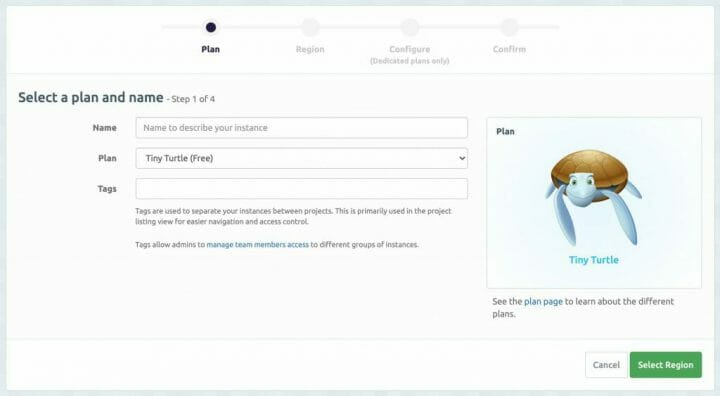
\includegraphics[scale=0.5]{imagens/nodejs-postgresql.jpg}
	\caption{
		Criação da primeira instância
	}
	\label{fig:instancia_01}
\end{figure}

Após adicionar um nome, selecione a região (não é necessário alterar), revise os dados e clique em \textit{Criar Instância}. Quando terminar, clique no nome da instância criada você terá acesso às credenciais de acesso e todas as seções que utilizaremos para manipular nosso banco. 

Para criar nossa primeira tabela, clique em \textit{Browser} e será aberto o \textit{SQL Browser}. Nele vamos digitar nossos comandos SQL.

\subsection{Comando CREATE TABLE no PostgreSQL}

O comando \textbf{SQL CREATE TABLE} é utilizado para definir uma nova tabela, inicialmente vazia (sem nenhum registro), no esquema de banco de dados atual. A tabela criada pertence ao usuário que executa o comando. Vejamos a sintaxe básica para a criação de uma tabela no postgres:

\begin{minted}[frame=single,framesep=10pt,breaklines,linenos,tabsize=2]{sql}
	CREATE TABLE [IF NOT EXISTS] nome_tabela (
		nome_coluna tipo_dados [COLLATE colecao] constraint,
		nome_coluna tipo_dados constraint,
		nome_coluna tipo_dados constraint,
		...,
		[FOREIGN KEY chave_estrangeira REFERENCES coluna]
		[ON DELETE acao ] [ ON UPDATE acao ]
	)
\end{minted}

Vamos criar uma tabela \textbf{autores} que irá conter os campos \textbf{id} \textbf{nome}, \textbf{sobrenome} e \textbf{datanascimento}

\begin{minted}[frame=single,framesep=10pt,breaklines,linenos,tabsize=2]{sql}
	CREATE TABLE autores (
		id SERIAL CONSTRAINT pk_id_autor PRIMARY KEY,
		nome varchar(30) NOT NULL, 
		sobrenome varchar(40) NOT NULL,
		datanascimento date
	);
\end{minted}

Agora, vamos criar a tabela de livros, incluindo os relacionamentos com as demais tabelas por meio do uso de chaves estrangeiras.

\begin{minted}[frame=single,framesep=10pt,breaklines,linenos,tabsize=2]{sql}
	CREATE TABLE livros (
		id SERIAL CONSTRAINT pk_id_livro PRIMARY KEY,
		nome varchar(50) NOT NULL,
		autor integer NOT NULL,
		editora integer NOT NULL,
		datapublicacao date,
		preco money,
		FOREIGN KEY (autor) REFERENCES autores (id) ON DELETE CASCADE
	);
\end{minted}

Outra forma de estabelecer esse relacionamento é simplesmente indicar a referência de uma coluna em sua própria declaração, o que a torna uma chave primária. Neste exemplo poderíamos escrever simplesmente:

\begin{minted}[frame=single,framesep=10pt,breaklines,linenos,tabsize=2]{sql}
	CREATE TABLE livros (
		id SERIAL CONSTRAINT pk_id_livro PRIMARY KEY,
		nome varchar(50) NOT NULL,
		autor integer REFERENCES autores(id) NOT NULL,
		editora integer NOT NULL,
		datapublicacao date,
		preco money
	);
\end{minted}

\subsection{Exercícios de fixação}
\noindent
\textbf{Crie as seguintes tabelas com seus respectivos relacionamentos:}

\noindent
\textbf{Empregado} (id:Serial, matricula:integer, cpf:varchar, nome:varchar, endereço:varchar, cep:integer) \\
\textbf{Projeto} (id:Serial, nom:varchar, verba:money) \\
\textbf{Alocação} (id:Serial, projeto:\textbf{foreingkey}, empregado:\textbf{foreingkey})

\begin{enumerate}
	\item Escreva o código antes de adicionar ao banco
	\item Valide o código com o professor 
	\item Adicione o código ao banco
\end{enumerate}

\section{Usando Node.js com o PostgreSQL}

Para iniciarmos nossa jornada com Node.js e PostgreSQL, vamos criar nosso primeiro projeto usando o \textbf{express.js}. Para maiores detalhes, acesse o link para relembrar sobre o funcionamento do \textit{Express Generator} \url{https://expressjs.com/pt-br/starter/generator.html}. Se, estiver usando o \url{https://replit.com} use o comando abaixo

\begin{minted}[frame=single,framesep=10pt,breaklines,linenos,tabsize=2]{javascript}
	npx express --view=ejs .	
\end{minted}

Contudo, para facilitar nosso trabalho, vamos realizar um \textit{fork} do seguinte repositório \url{https://github.com/luizpicolo/skeleton-nodejs-express-ejs.git} e importá-lo no \textbf{replit}.

\subsection{Conexão com o banco de dados}

Assim, após todo o processo ter ocorrido sem erros, vamos configurar a conexão com o banco. Crie um arquivo \textbf{db.js} na raiz do seu repositório.Não podemos criando conexões infinitas no banco pois isso, além de ser lento, é inviável do ponto de vista de infraestrutura. Usaremos aqui um conceito chamado \textit{connection pool}, onde um objeto irá gerenciar as nossas conexões, para abrir, fechar e reutilizar conforme possível. Vamos guardar este único pool em uma variável global, que testamos logo no início da execução para garantir que se já tivermos um \textit{pool}, que vamos utilizar o mesmo.


\begin{minted}[frame=single,framesep=10pt,breaklines,linenos,tabsize=2]{javascript}
	let connect = function() {
		if (global.connection){
			return global.connection.connect();
		}
		
		const { Pool } = require('pg');
		const pool = new Pool({
			connectionString: 'URL PARA O BANCO DE DADOS'
		});
		
		global.connection = pool;
		return pool.connect();
	}
	
	module.exports = { connect };
\end{minted}

Para que o código acima funcione corretamente, devemos instalar a dependência \textbf{pg}, executando o comando abaixo. 

\begin{minted}[frame=single,framesep=10pt,breaklines,linenos,tabsize=2]{javascript}
	npm i pg --save	
\end{minted}

\subsection{Criando nosso primeiro modelo para acesso ao dados}

Para que possamos testar a conexão com o banco em nossos modelos, vamos criar um modelo de exemplo chamado \textbf{Autor} e invocar o código de conexão da seguinte forma.

\begin{minted}[frame=single,framesep=10pt,breaklines,linenos,tabsize=2]{javascript}
const db = require("../db");

class Autor { 

}

module.exports = Autor;
\end{minted}

Usando apenas a chamada acima, já possuímos um modelo que pode obter os dados necessários por meio de uma conexão com o banco de dados. 

\subsection{As quatro operações básicas em um banco de dados}\label{sub:crud}

Nas manipulações de registros realizadas diretamente em banco de dados ou em plataformas desenvolvidas no padrão \textit{RESTful}, o conceito \textbf{CRUD} estabelece o modelo correto no manuseio desses dados.

CRUD representa as quatro principais operações realizadas em banco de dados, seja no modelo relacional (SQL) ou não-relacional (NoSQL), facilitando no processamento dos dados e na consistência e integridade das informações.

A sigla CRUD significa as iniciais das operações create (criação), read (leitura), update (atualização) e delete (exclusão). Essas quatro siglas tratam a respeito das operações executadas em bancos de dados relacional (SQL) e não-relacional (NoSQL). Essas operações pertencem ao agrupamento chamado de \textit{Data Manipulation Language (DML)}, utilizado na linguagem Structured Query Language (SQL)\footnote{Para mais detalhes acesse: \url{https://blog.betrybe.com/tecnologia/crud-operacoes-basicas/}}.

\subsubsection{Create}

A operação de criação de um registro em uma tabela é realizada pelo comando INSERT. Exemplo:

\begin{minted}[frame=single,framesep=10pt,breaklines,linenos,tabsize=2]{python}
class Autor {
	static async insert(data){
		const connect = await db.connect();
		const sql = 'insert into autores(nome, sobrenome, datanascimento) values ($1, $2, $3);';
		const values = [data.nome, data.sobrenome, data.datanascimento];
		return await connect.query(sql, values);
	}
}
\end{minted}

\subsubsection{Read}

A operação de consulta de um ou mais registros em uma tabela é realizada pelo comando SELECT. Exemplo:

\begin{minted}[frame=single,framesep=10pt,breaklines,linenos,tabsize=2]{javascript}
static async select(){
	const connect = await db.connect();
	return await connect.query('select * from clientes');
}
\end{minted}
\subsubsection{Update}

Comando utilizado para a atualização de um ou mais registros de uma tabela. Exemplo:

\begin{minted}[frame=single,framesep=10pt,breaklines,linenos,tabsize=2]{javascript}
static async update(id, data){
	const connect = await db.connect();
	const sql = 'UPDATE clientes SET nome=$1, idade=$2, uf=$3 WHERE id=$4';
	const values = [data.nome, data.idade, data.uf, id];
	return await connect.query(sql, values);
}
\end{minted}
\subsubsection{Delete}

Comando utilizado para a exclusão de registro (s) de uma tabela. Exemplo:

\begin{minted}[frame=single,framesep=10pt,breaklines,linenos,tabsize=2]{javascript}
static async delete(id){
	const connect = await db.connect();
	const sql = 'DELETE FROM clientes where id=$1;';
	return await connect.query(sql, [id]);
}
\end{minted}

\subsection{Invocando os métodos nas rotas}

Para que possamos invocar os métodos de manipulação de dados do modelo, precisamos criar uma rota. Para tanto, crie uma nova rota utilizando o \textbf{express} e adicione a seguinte rota para que seja feita a seleção dos dados.

\begin{minted}[frame=single,framesep=10pt,breaklines,linenos,tabsize=2]{javascript}
var express = require('express');
var router = express.Router();
// Invocando o modelo Autor
const Autor = require("../models/autor");

/* Listando os usuários e apresentando um Json */
router.get('/', async function(req, res, next) {
	const data = await Autor.select();
	res.json(data.rows);
});

module.exports = router;
\end{minted}